\documentclass[10pt]{article}
\usepackage[final]{graphicx}
\usepackage{amsfonts}
\usepackage{amsmath}
\usepackage{caption}
\usepackage{subcaption}

\topmargin-.5in
\textwidth6.6in
\textheight9in
\oddsidemargin0in

\def\ds{\displaystyle}
\def\d{\partial}

\begin{document}

\centerline{\large \bf Given a helical compression spring in a spring-mass-damper system, what are optimal springs?}

\vspace{.1truein}

\def\thefootnote{\arabic{footnote}}
\begin{center}
  Justin Krueger\footnote{Mathematics, Virginia Tech University},
  Alistair Bentley\footnote{Mathematics, Clemson University},
  Tianyu Qiu\footnote{Mathematics, University of Delaware},
  Saideep Nannapaneni\footnote{Civil \& Environmental Engineering,Vanderbilt University},
  Jiahua Jiang\footnote{Mathematics, University of Massachusetts Dartmouth },
  Tim Hodges\footnote{Mathematics, Colorado State University}
\end{center}

%\vspace{.1truein}

\begin{center}
Problem Presenters: Jordan Massad \footnote{Sandia National Laboratory},
Sean Webb \footnote{Sandia National Laboratory},
	Faculty Mentors: Ilse Ipsen\footnote{North Carolina State University},
	Ralph Smith\footnote{North Carolina State University}, 
\end{center}


\vspace{.3truein}
\centerline{\bf Abstract}






\section{Introduction}
%It should be written as much as possible in non-technical terms, so that a
%lay reader can understand the context and the contribution of the paper.

The use of mechanical switches in industry is a cornerstone of the modern world. Many mechanical switches are designed to use a spring. Depending on the use of the switch, the spring can be optimized for the function of the spring. 

For example, consider an acceleration switch in figure \ref{Acceleration Switch}. 

		\begin{figure}[h]
		 \begin{center}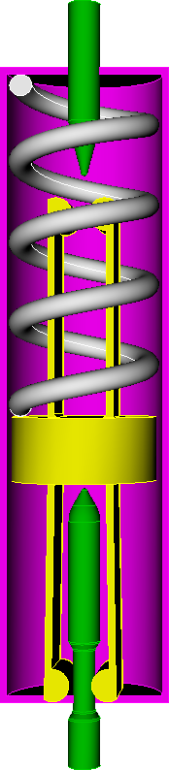
\includegraphics[scale=.2]{Acceleration_Switch.png}\end{center}
		 \caption{An example of an acceleration switch}
		 \label{Acceleration Switch}
		 
		 \end{figure}
		 
		
\textbf{Describe problem, approach, and summarize contribution and results.}
This switch is used in high acceleration testing. The use is to only record information at crucial times of the test. For this reason when a certain force is exerted on the switch the pins at both ends will connect. When this happens we have a circuit that will enable data collection. It is important that the switch does not open too soon or too late otherwise the data collection will be too large or too little.This is just one example of a switch that we must know the best spring to make the performance maximal. For a more in depth look at this example look at \cite{IMSM2010}

Given that a switch may be used in a myriad of ways, it is important that one can find an optimal spring, after the use of the spring is known. This leads to an optimization problem. Even more this leads to an optimization problem that requires flexibility to allow how a spring is determined to be optimal. In other words, the objective function and constraints must be interchangeable. In addition there are fabrication constraints that exist during manufacturing to consider.  

Given any constraint or objective function it will depend on a set of variables. In optimization we only wish to concern ourselves with the state variables that are allowed to change during optimization. For this reason, we construct a spring object that will hold all attributes of a spring and we can pull the relevant variables when it is determined what they are. 

In addition to this spring object, to reduce the uncertainty of the problem we conduct a sensitivity analysis of the objective function subject to the constraints and variables given. Allowing the user to reduce the state variables if it is determined that for a set of variables given there exist insensitive state variables. 

A main contribution of this work is the framework to add constraints and objectives that may be unknown at the point of this paper. In parallel to this we have built a framework that is flexible enough to address the issue of unknown constraints and objectives. \textbf{ADD!}


\textbf{review history and existing literature}
Designing an optimal spring is not a new problem. In 2010 at the SAMSI IMSM workshop a team considered the design of an acceleration switch with enabled uncertainty. In fact, the switch they considered was in figure \ref{Acceleration Switch}. This approach lead to a paper \cite{IMSM2010}. This is not the only approach to uncertainty, in \cite{Reliability} probabilistic response surface methodology was implemented to investigate the complications of uncertainty in designing a spring. In addition to these types of approaches it is possible to narrow focus to a single parameter, in \cite{Robust} they focus on the spring stiffness. In \cite{Paredes} they attempt to design an optimal spring, with the introduction of a sizing tool. All references listed are informed to some extent by \cite{Wahl}. 

Our approach is not limited to an acceleration switch, instead it is but a special case of our approach. We do not focus on a set of parameters or attempt to fix the uncertainty of the spring design problem initially. We attempt to allow any possible construction of a spring optimization possible. 

This does not rule out if a construction is not physically or mathematically invalid. We will dispose of that case when we are unable to find a feasible point for optimization within our feasibility check. In summary, we need to allow any possible construction of a spring design problem, and adjust accordingly. 


\textbf{outline}
In this paper we will give a description of the springs of interest, helical compression springs. Next, the formulation of the problem, and the approach taken to the problem. Following will be a section on workflow with descriptions of each step in the workflow. Lastly, we will discuss a few case studies given the framework constructed and a summary with future work that can be worked on.





\section{Helical Compression Springs}

Helical springs are the typical spring that comes to most peoples mind, for illustrative purposes, see figure \ref{Spring}. 

		\begin{figure}[h]
		 \begin{center}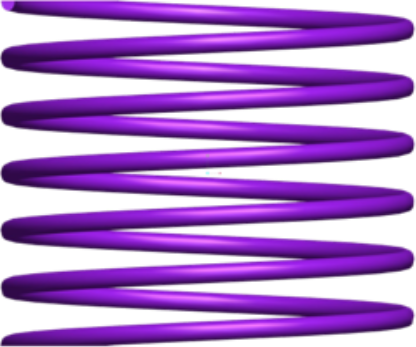
\includegraphics[scale=.2]{Spring.png}\end{center}
		 \caption{An example of a helical compression spring.}
		 \label{Spring}
		 
		 \end{figure}

Below is a list of a spring's key design parameters. We have added a few illustrations to illustrate some of the parameters. 		 
		\begin{figure}[h]
			\centering
			\begin{subfigure}{.5\textwidth}
				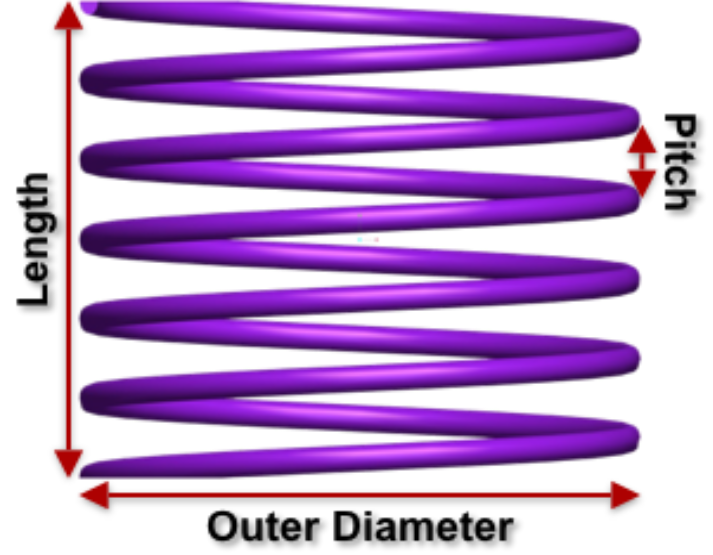
\includegraphics[scale=.2]{Spring_Description.png}
				\caption{Pitch, outer diameter, and length of a spring.}
				\label{Description1}
			\end{subfigure}%
			\begin{subfigure}{.5\textwidth}
				  \centering
		 		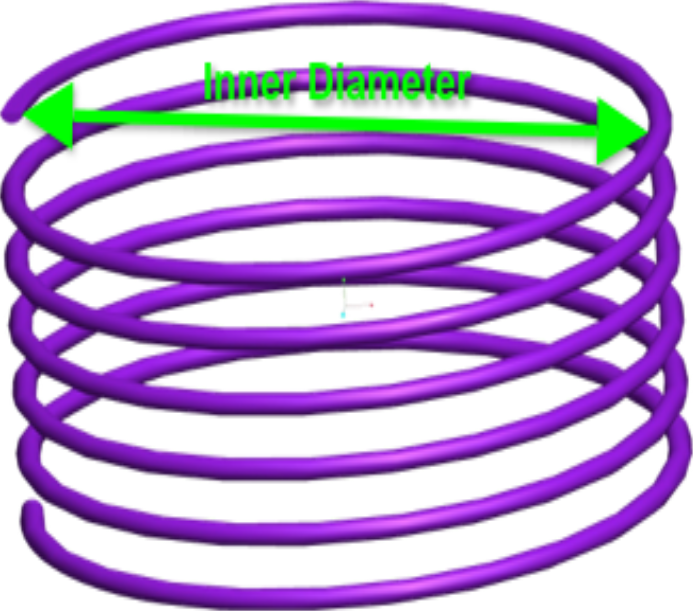
\includegraphics[scale=.2]{Spring_Description2.png}
				\caption{Inner diameter}
				  \label{Description2}
		  		
			\end{subfigure}
			 \label{Descriptions}
		  \caption{A few illustrations of parameters for a helical compression spring.}
		\end{figure}
		
		\begin{enumerate}
			\item Spring's inner diameter $d_{i}$, illustrated in figure \ref{Description2}.
			\item Spring's outer diameter $d_{o}$ illustrated in figure \ref{Description1}.
			\item Spring's wire diameter $d_{w}$.
			\item Total number of spring coils $N_{t}$.
			\item Active number of spring coils $N_{a}$, active coils are not touching any other coils, and is subject to the spring being closed or open. 
			\item Pitch $p$ illustrated in figure \ref{Description1}.
			\item Spring's free length $L_{free}$, the spring's length without any force applied. 
			
			\item Spring's solid length $L_{solid}$, the spring's length when all coils are compressed together.
			\item Spring's open length $L_{open}$, the spring's length at open position, open is beginning state.
			\item Spring's open length $L_{close}$, spring length at close position, close is the ending state.
			\item Spring's open length $L_{hard}$, the maximum a spring can compress for the application.
			\item Spring's open force $F_{open}$, this is the force on the spring in open position.
			
			
			\item Spring's shear modulus $G$, this is determined by the material of the spring.
			\item Spring's youngs modulus $E$, this is determined by the material of the spring.
			\item Spring's poisson ratio $\nu$, this is determined by the material of the spring.
			\item Ultimate torsional stress, UTS. 
		
		\end{enumerate}
		
		In addition to these parameters there are the following attributes that are empirical. We care about these attributes within some regime. This is because outside of certain conditions these attributes exhibit special behavior. 
		
			%\begin{enumerate}
			%	\item 
			Spring Rate:\begin{equation} k = \frac{G}{8N_{a}}\frac{d_{w}^{4}}{(d_{i} + d_{w})^{3}}\end{equation}
				
				 Spring Index:\begin{equation}C = \frac{d_{i}}{d_{w}} + 1.\end{equation}
				
				Coil Binding Gap\begin{equation} g = \frac{L_{hard} - L_{solid}(d_{w},N_{a}; ec)}{N_{t} - 1}\end{equation}
		
				 Max Shear Stress\begin{equation} \frac{G(L_{free} - L_{hard})}{4 \pi N_{a} (ec)} \left[\frac{d_{w} (4d_{i}^{2} + 9.46d_{i} 
d_{w} + 3 d_{w}^{2})}{d_{i}(d_{i}+d_{w})^{3}}\right]< UTS\end{equation}
		
				Diametral Expansion\begin{equation} d_{expand} = d_{w} + \sqrt{(d_{i} + d_{w})^{2} + \frac{p^{2} - d_{w}}{\pi^{2}}}
			\end{equation}
			
\section{The Problem} 

Design an algorithm that optimizes springs with interchangeable objectives and constraints. In addition, attempt to incorporate properties stress relaxation and creep into the available objectives and constraints. 

A list of possible constraints/objectives given in minimization form is below

\begin{enumerate}
\item $d_{i} < d_{i}^{max}$
\item $d_{i} < d_{o}$
\item $d_{i} + 2d_{w} < d_{o}^{max}$
\item$d_{expand} - d_{0}^{max} < 0 $
\item$ \frac{G}{8N_{a}}\frac{d_{w}^{4}}{(d_{i} + d_{w})^{3}} - k_{max} \le 0 $
\item $\frac{d_{i}}{d_{w}} + 1 - C_{max}< 0$
\item $(L_{free} - L_{open})\frac{G}{8N_{a}}\frac{d_{w}^{4}}{(d_{i} + d_{w})^{3}} - F_{open} = 0 $
\item $\frac{L_{hard} - L_{solid}}{N_{t} - 1} + g_{min} \le  0$
\item$\frac{L_{free}}{d_{i} + d_{w}} - \pi \sqrt{\frac{2(2 \nu + 1)}{\nu + 2}}$
\item$-UTS + \frac{G(L_{free} - L_{hard})}{4 \pi N_{a} (ec)} \left[\frac{d_{w} (4d_{i}^{2} + 9.46d_{i} 
d_{w} + 3 d_{w}^{2})}{d_{i}(d_{i}+d_{w})^{3}}\right] < 0$
\end{enumerate}	

This list is not exhaustive as we want a user to be able to define new constraints and objectives. 
In addition to these we should be able to minimize any parameter of the spring. 


\textbf{ADD RELAXATION HERE!}




In order to simplify the problem we have made some assumptions. First, we have assumed that constraints and objectives are all in terms of the number of total coils. This is to reduce the complexity of knowing if a constraint is dependent on the active number or total number of coils. These two numbers are dependent on the end conditions of the spring, whether it is open or closed at the end. 

For simplicity we also will consider all springs to be have a closed end condition. With these assumptions we simplify our constraints for pitch, $p$, solid length, $L_{solid}$, and the diametral expansion, $d_{expand}$. 

\textbf{JUSTIFY ASSUMPTIONS}

\textbf{Describe your data, how you collected them, their properties,
and whether you did 
anything to them (removed noise, filled in missing data, 
applied normalizations).}

\section{The Problem}
\begin{itemize}
\item Give a precise technical description of your problem. 

\item State and justify all your assumptions. 

\item Define notation. 

\item Describe your data, how you collected them, their properties,
and whether you did 
anything to them (removed noise, filled in missing data, 
applied normalizations).
\end{itemize}


\section{The Approach}

To be as flexible as possible we must be able to handle constraints and objectives that have an unknown number of  variables a priori. To handle this uncertainty we instead of evaluating an objective or constraint with a set of values we evaluate with a "spring object" in the programming sense \cite{OOP}. This spring has all the attributes of interest and the function merely picks what values it needs for evaluation. 

This approach is also implemented in the design of a constraint and objective. An objective is an expression that we must be able to evaluate. A constraint is an expression that we must evaluate and check if this evaluationa violates the constraint condition. We use the idea of inheritance and let a constraint inherit the properties of being an objective with additional framework to compare to a condition. This allows the user to interchange constraints and objectives seamlessly.

Along with the flexible software design, we have implemented the ability to run feasibility and sensitivity checks before trying to optimize. This will allow the user to know additional information about the problem. First, from feasibility, the user will know quickly if the run is unable to find a feasible point to run optimization. Second, from sensitivity, the user can know which parameters will dramatically change the optimization versus which parameters are unnecessarily adding to the dimension of the optimization space. 
 

\section{The Approach}
\begin{itemize}
\item Present and justify your approach for solving the problem. 
\item Explain the advantages of your approach over existing ones.

\item Tell a story.
Don't just say: ``I did this, then I did this, and at last I did this''.
\end{itemize}
\newpage
\section{Workflow}
 		\begin{figure}[h!]
		 \begin{center}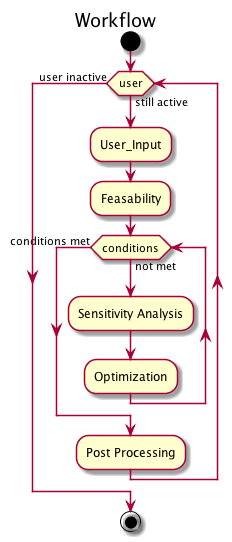
\includegraphics[scale=.4]{IMSM_Workflow.png}\end{center}
		 \caption{Illustration of the flow of our approach.}
		 \label{Workflow}
		 
		 \end{figure}
Above is an illustration of the workflow that is our approach. This section will go in depth into the feasibility, sensitivity analysis and optimization of our approach.

\subsection{Feasibility}

\subsection{Sensitivity Analysis}
\hspace{5 mm} As the dimension of design variable space increases, the computational expense of the optimization procedure increases. To reduce the computational expense, it is often desirable to reduce the design variable space by removing the variables that have very little influence on the objective function. Thus, a dimension reduction strategy is required to reduce the design variable space. Dimension reduction approaches, in the literature have been divided into two categories - (1)filter approach, and (2)wrapper approach. In the filter approach, the input variables are ranked according to a ranking criterion and the most dominant variables can be selected by assuming a threshold influence value. In the wrapper approach, a subset of variables is selected from the list of all possible subsets of the input variables that best estimate the output variable. An optimization technique is used to obtain the best subset of input variables. In this work, the variance-based Global Sensitivity Analysis (GSA), a filter approach, is used for dimension reduction. Note that the input variables represent the design variables for the objective function. 

\hspace{5 mm} Consider a objective function, $G$, with $n$ design variables given by $x_{1}$, $x_{2}$, ...  $x_{n}$, given by

\centerline{$Y = G(x_{1}, x_{2}, ... x_{n})$}

In GSA, two types of indices can be calculated for each variable - first order index and total effects index. The first-order index ($S_{i}^{I}$) quantifies the uncertainty contribution of an input variable, without considering its interactions with other variables, to the output variable uncertainty. Similarly, the total effects index ($S_{i}^{T}$) quantifies the uncertainty contribution of an input variable by considering its interactions with all variables, to the output uncertainty. The expressions for the two sensitivity indices are given below as 

\centerline{$S_{i}^{I} = \frac{V_{X_i}(E_{X_{-i}}(Y|X_{i}))}{V(Y)}$}
\centerline{$S_{i}^{T} = \frac{E_{X_{-i}}(V_{X_{i}}(Y|X_{-i}))}{V(Y)}$}

Given a design range (lower and upper bounds), a variable can be assumed to be uniformly distributed in the design range. For each variable, the total-effects index is calculated and if it is less than an assumed threshold value, then that variable is assumed insensitive and removed from the optimization procedure. Thus, dimension reduction is implemented for a faster design optimization.\cite{Bioinformatics} \cite{Wrappers} \cite{Error} \cite{Global}
\subsection{Optimization}
\cite{Derivative} \cite{DirectPaper} \cite{MATLAB:2014a} \cite{DirectUserGuide}
 
 

\section{Computational Experiments}
\subsection{Basics about uni-axial creep and stress relaxation}
The spring is heated to $0.3-0.5T_m$ ($T_m$ is the melting temperature of the material) and loaded by a tensile force. The induced normal stress $\sigma$ is much less than the yield limit of the material $\sigma_y$. The load and temperature are constant throughout the test. The strain $\epsilon^{cr}$ will slowly increase.

Conventionally, creep can be divded into $3$ stages. In the first stage(primary/reduced/trasient) ,the creep strain rate decreases to a certain value(minimum creep rate). The second stage(secondary/steady/stationary creep) is characterized by a nearly constant creep rate(minimum creep rate). In the third stage(tertiary creep), the creep strain rates increases rapidly and leads to rupture. The first stage is usually reversible with time after unloading, while the second/third ones are not. Since the primary creep occurs in a short duration and the tertiary one leads quickly to rupture, the secondary creep is under most serious consideration in many design in many engineering applications.

Stress relaxation is the phenomenon that the stress decreases when the strain is held constant in time. During the test the load is continuously decreased in such a way that the initial strain remains constant.

\subsection{Creep rate law of material}
The starting point is the assumption that the creep rate may be described as a product of two separate functions of stress, temperature and time
\[
\epsilon^{cr}=f_\sigma (\sigma) f_T(T) f_t(t)
\]
The widely used functions of stress $f_\sigma(\sigma)$ are:

\begin{tabular}{ll}
$a\sigma^n$ & Norton, 1929, Bailey, 1929 \\
$b\left( \exp{\sigma\over \sigma_0} -1 \right)$ & Soderberg, 1936 \\
$a\mathop{sinh}{\sigma\over \sigma_0}$ & Prandtl, 1928, Nadai, 1938, McVetty, 1943\\
$a_1\sigma^{n_1} + a_2 \sigma^{n_2}$ & Johnson et al., 1963 \\
$a\mathop{sinh} \left( {\sigma\over \sigma_0}\right)^n$ & Garofalo, 1965
\end{tabular}

where $a,b,a_1,a_2,\sigma_0,n_1,n_2$ are material constants that could depend on time $t$. The dependence on the temperature $f_T(T)$ is usually expressed by the Arrhenius law
\[
f_T(T) = \exp \left( {-Q\over RT}\right)
\]
where $Q$ and $R$ denote the activation energy and the Boltzmann's constant.

The time dependence part $f_t(t)$ is

\begin{tabular}{ll}
$t$ & secondary creep \\
$bt^m$ & Bailey \\
$(1+bt^{1/3})\exp{kt}$ & Andrade\\
$\sum_j a_j t^{m_j}$ & Graham and Walles
\end{tabular}

For simplicity, we are going to only use the Norton-Bailey law.
\subsection{Stress relaxation of helical spring}
Due to conservation of the total shear strain, the sum of the creep strain $\epsilon^{cr}$'s rate of change and that of elastic shear strain $\epsilon_{el}$ is zero:
\[
\dot{\epsilon}_{cr} + \dot{\epsilon}_{el} = 0
\]
The elastic shear strain is related to the shear stress by shear modulus $G$:
\[
\epsilon_{el} = \sigma/G
\]
and therefore
\[
\dot{\epsilon}_{el} = \dot{\sigma}/G
\]
According to Norton-Bailey law(also known as time hardening law),
\begin{equation} \label{eq:N-B}
\dot{\epsilon}_{cr}(t)=c\sigma^{n+1} t^{k-1}
\end{equation}
where $c$ is the shear strain rate, $n,k$ are temperature dependent material constants.

Substituting the above two equations to the conservation law,
\begin{equation} \label{eq:diff}
\dot{\sigma}(t)/G+c\sigma(t)^{n+1} t^{k-1}=0
\end{equation}
The initial condition is
\[
\sigma (0) = G\theta r
\]
where $\theta$ is the initial twist angle per unit length, $r$ the radius of wire.

\[
\sigma = \left( (G\theta r)^{-n} + {c\over k} Gnt^k \right)^{-{1\over n}}
\]

The torque can be written as
\[
M(t) = 2\pi \int_0^{d_w} r^2 \sigma(r,t)\,\mathrm{d} r ={}_{2}F_1 \left( {4\over n},{1\over n};{4+n\over n};{c\theta^n G^{n+1} n t^k\over k} {d_w^n\over 2^n}\right) M(0)
\]
where $d_w$ is the wire diameter.

Since the spring load is linearly related the torque $P_z(t)\propto M(t)$, given the constant deflection $s$,
\[
{P_z(t)\over P_z(0)} = {}_{2}F_1 \left( {4\over n},{1\over n};{4+n\over n};{c\theta^n G^{n+1} n t^k\over k} {d_w^n\over 2^n}\right)
\]
where
\[
\theta = {2s\over \pi N_a ((d_i+d_o)/2)^2}
\]
The closer this quantity is to $1$, the better the spring quality is.

\subsection{Creep of helical spring}
The starting point is still the Norton-Bailey law (\label{eq:N-B}). There is naturally another way to write the shear strain rate:
\[
\dot{\epsilon}^{cr} = \dot{\theta} r = {8\dot{s} r\over \pi N_a (d_i+d_o)^2}
\]
We obtain $\sigma$ from substiting the above equation into Norton-Bailey law. Given the constant spring force $P_z^0$,
\[
P_z^0{d_i+d_o\over 4}=M(0)=2\pi\int_0^{d_w} r^2 \sigma(r,t)\,\mathrm{d} r
={\pi\over 4}{n+1\over 4+3n}\left( {8d_w^{4+3n}\dot{s} \over t^{k-1} (d_i+d_o)^2 \pi N_a c (d_i+d_o)^2} \right)^{{1\over n+1}}
\]
It can be deduced that the spring length $s$ follows
\[
s(t) = s(0) + \left( {(d_i+d_o)P_z^0\over \pi}{4+3n\over n+1} \right)^{n+1} {\pi (d_i+d_o)^2 N_a c\over 8kd_w^{4+3n}} t^k
\]
where $s(0)$ is the initial spring length. The less the difference of the spring length $s(t)-s(0)$, the better the spring quality is.

Give enough details so that readers can duplicate your experiments.

\begin{itemize}
\item Describe the precise purpose of the experiments, and what they 
are supposed to show.

\item Describe and justify your test data, and any assumptions you made to 
simplify the problem.

\item Describe the software you used, and the 
parameter values you selected.

\item 
For every figure, describe the meaning and units of the coordinate axes, 
and what is being plotted.

\item Describe the conclusions you can draw from your experiments
\end{itemize}

\section{Summary and Future Work}
The ability to interchange constraints and objective functions with any number of design variables allows the user the utmost flexibility. With the addition of feasibility and sensitivity analysis it is possible for any configuration of objective function, constraints, and design variables to be analyzed for refinement. The quantification of stress relaxation and creep allow the user a chance to incorporate these properties into any configuration, especially those that have never been tested. 

Some limitations of the approach outlined are as follows. The choice of optimization and sensitivity analysis are fixed, however, they are modularized to allow a different optimization routine and sensitivity analysis to be ported in. Given the amount of flexibility that is enabled, a user will have to be able to decide if a infeasible solution is due to user error. 

Future work is bountiful for this approach. More analysis of the stress relaxation and creep could result in better performance. An in depth analysis of different models of stress relaxation and their performance in our model would be beneficial. 



\vfill\pagebreak

	
	\bibliographystyle{ieetr}

\bibliography{MyBib}



\end{document}

